\subsection{Numerical Experiments}
    
    Now, we will proceed to describe the steps necessary to implement the method based on the above:
    \begin{enumerate}
    	\item We are going to consider the interval given by $[0, 1]$, which represents the domain of physical space, and similarly, the time will be set by the real value $t_f>0$ such that $[0, t_f]$. So, as a first step, we must define the problem well by choosing the parameters identified and required by the problem \ref{infinite_system}, which in the same way will be denoted by: $N$, $M$, $N_1 \in \mathbb{N}$, and $\alpha \in \mathbb{R}^+$.
    	
    	\item Given the above information, it is possible to follow the same methodology that we have analyzed in \ref{finite_system}, and define as a second step the calculation of the set $J^{M, N}$ given by \ref{Conjunto_J}, and then, as an intermediate step, obtain the set of points for each domain that we have defined above. 
    	
    	As an observation, the choice of the set of points, in this case, is arbitrary, and for example, We could obtain them by calculating the points $\xi_i \in [0, 1]$ defined for each $i = 0, 1, \dots, p \in \mathbb{N}^+$ as
    	\begin{align*}
    		\xi_i = \xi_0 + i \Delta \xi, \hspace{2mm} i = 0, 1, \dots, p
    	\end{align*}
    	and similarly for $t_j \in [t_0, t_f]$ with $j = 0, 1, \dots, l \in \mathbb{N}^+$ to obtain the following
    	\begin{align*}
    		t_j = t_0 + j \Delta t, \hspace{2mm} \Delta t = \frac{t_f - t_0}{l} 
    	\end{align*}
    	
    	\item Concluding with the previous steps will allow us to obtain everything that is required to begin to construct the initial value problem of the system \ref{finite_system_vectorial}, which could be considered as the step that requires more attention because we must obtain the matrix $\bar{C}_{n, m}$ using the simplification given in \ref{Cnm}. 
    	
    	However, this calculation gives the impression that it will give us a lot of work, but when observing its expression we can notice that we only have to focus on each of the combinations given by the multiplication of the Hermite polynomials that we must then integrate, for example, using some quadrature rule, and finally make its summation.
    	
    	\item Successfully achieving this last step, what remains are to solve an eigenvalue problem given by \ref{eigen}, which is solved by some conventional numerical method to obtain the eigenvalues $\eta_i$ with their respective eigenvectors $V_i$. 
    	
    	Then, Using the functional $u_0$ as in \ref{IC_approx} to calculate the constants $c_k$ for each $k = 1, \dots, M$, and by using the expansion given by \ref{solution_finite_system} to obtain the solution of the problem as follows

    	\begin{align*}
    		u^M(x_i, t_j) = \displaystyle \sum_{k=1}^{M} u_k (t_j) H_k (x_i), \hspace{2mm} \left\{x_i\right\}_{i=0}^{p} \in \left[ 0, 1 \right], \left\{t_j\right\}_{j=0}^{l} \in \left[ 0, t_f \right]
    	\end{align*}
    \end{enumerate}
    
    The following simulations that will be shown were performed using a discretization of $2048$ points in the spatial variable $\xi$ over the interval $[0, 1]$, and $1024$ points in the variable time $t$ over the interval $[0, 10]$. In addition, the values of the parameters $N = 5$, $M = 11$, and $\alpha = 1.0 \times 10^{-2}$ were considered. With this information, the solutions obtained were calculated using the following initial condition and its truncated Chebysheb expansion given by
    \begin{align*}
    	x(\xi) = \sin(\pi \xi), \hspace{3mm} y(\xi) = \displaystyle \sum^{N}_{k=0} c_k T_k (\xi),
    \end{align*}
    
    This numerical experiment consists of illustrating an interesting result given in \cite{Delgado2019}, which tells us that the solutions obtained from two close initial conditions also remain close. This behavior allows characterizing what is known as the stability of the approximation, and it is described by means of continuity with respect to the initial conditions of the numerical approximations of the equation (\ref{kolmogorov}). \\
    
    To understand this better, let us denote by $\Psi^{x}_t$ the solution of (\ref{kolmogorov}) obtained by
    \begin{align*}
    	u(x, t) = \mathbb{E} \left[ \varphi (X^x_t) \right]. 
    \end{align*}
    where $\varphi: \mathcal{H} \rightarrow \mathbb{R}$ is Lipschitz and $X^x_t$ is the solution to (\ref{stochastic_equation}) with initial conditions $X_0 = x \in \mathcal{H}$. So, as before, its expansion is given by
    \begin{align*}
    	\Psi^{x}_t = \displaystyle \sum _{n \in \mathcal{J}} u_n (t) H_n (x), \hspace{2mm} x \in \mathcal{H}, \hspace{2mm} t \in [0, T].
    \end{align*}
    
    Therefore, following our reference, the above is summarized as follows: Given two different initial conditions $x, y \in \mathcal{H}$, then we have the following estimate
	\begin{align*}
		\| \Psi^x_t - \Psi^y_t \|^2_{\left( L^2 (\mathcal{H}, \mu)\right)^2} \leq \exp(Ct) \displaystyle \int_{\mathcal{H} \times \mathcal{H}} \|x - y \|^2_{\mathcal{H}} \mu (dx) \mu (dy) + f(t) \|x - y\|_{\mathcal{H}},
	\end{align*}
	for some $C$ finite and $f(t)$ is given by
	\begin{align*}
		f(t) = \displaystyle \sum_{n \in J} \left[u^y_n (t)\right]^2 + \int_{\mathcal{H}} \mathbb{E}^2 \left[\varphi (X^y_t)\right] \mu (dy).
	\end{align*}	
	
	From the above, we can see that if $ \| x - y \|_{\mathcal{H}} \leq \delta$, so we have to $\| \Psi^x_t - \Psi^y_t \| \leq G (t) \delta$. As we have already mentioned, this continuity defines a type of stability for approximations, which is of utmost importance in this field since characterizations of this type are still under construction and are essential for the analysis of a numerical method. \\
	
	This behavior is shown in the following figures, which were obtained using codes that were created following the previous steps, and which can be found in \url{https://github.com/alanmatzumiya/Paper.git}. In figure \ref{IC_Cheb} it shows us the two initial conditions for which the equation (\ref{kolmogorov}) will be solved by associating it with (\ref{burgers_stochastic}), and in figure \ref{Stochastic_Solutions} we can see that the solutions keep the distance. Finally, the figure \ref{Continuity} shows the distances for each instant of time $t$, showing that they are actually getting closer as time passes.
	
\newpage
	\begin{figure}[H]	
		\centering	
		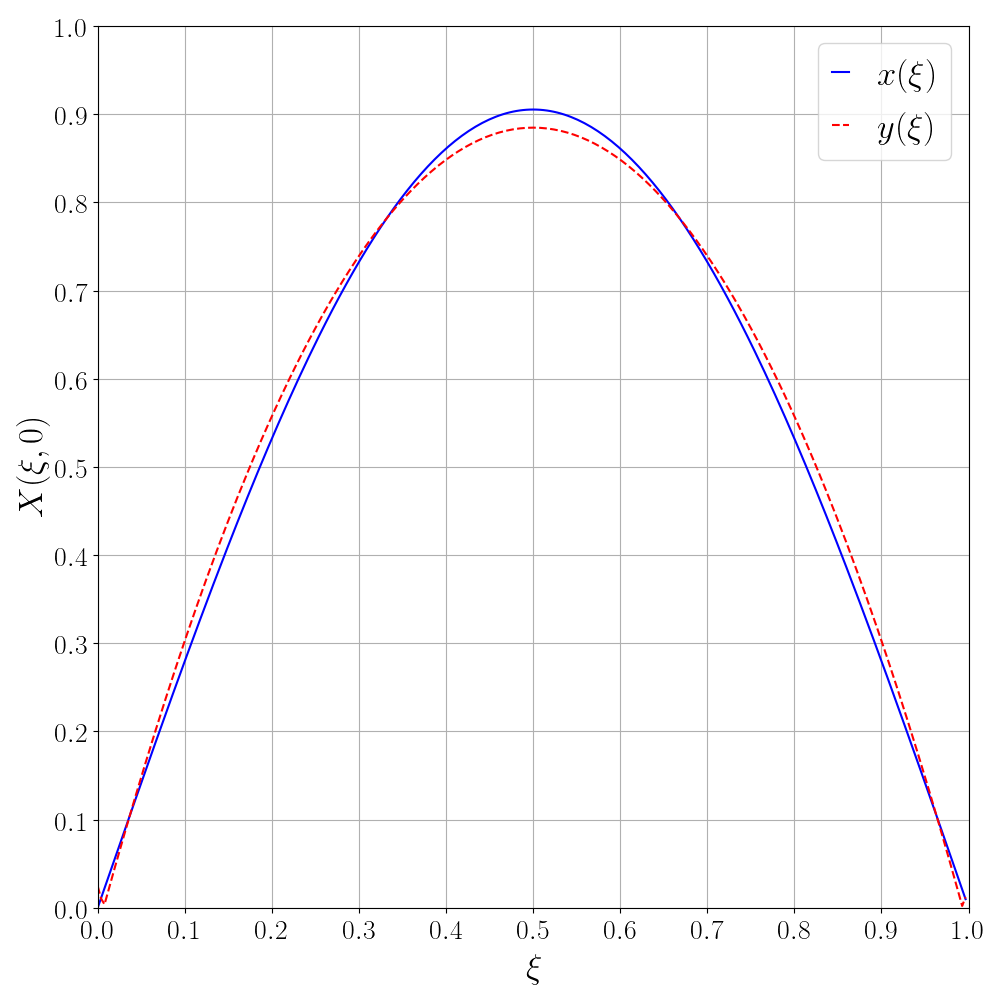
\includegraphics[width=.55\textwidth]{burgers_equation/stochastic/numerical_experiments/figures/IC.png}
		\caption{Initial condition for (\ref{burgers_stochastic2}) and its approximation.}
		\label{IC_Cheb}	
		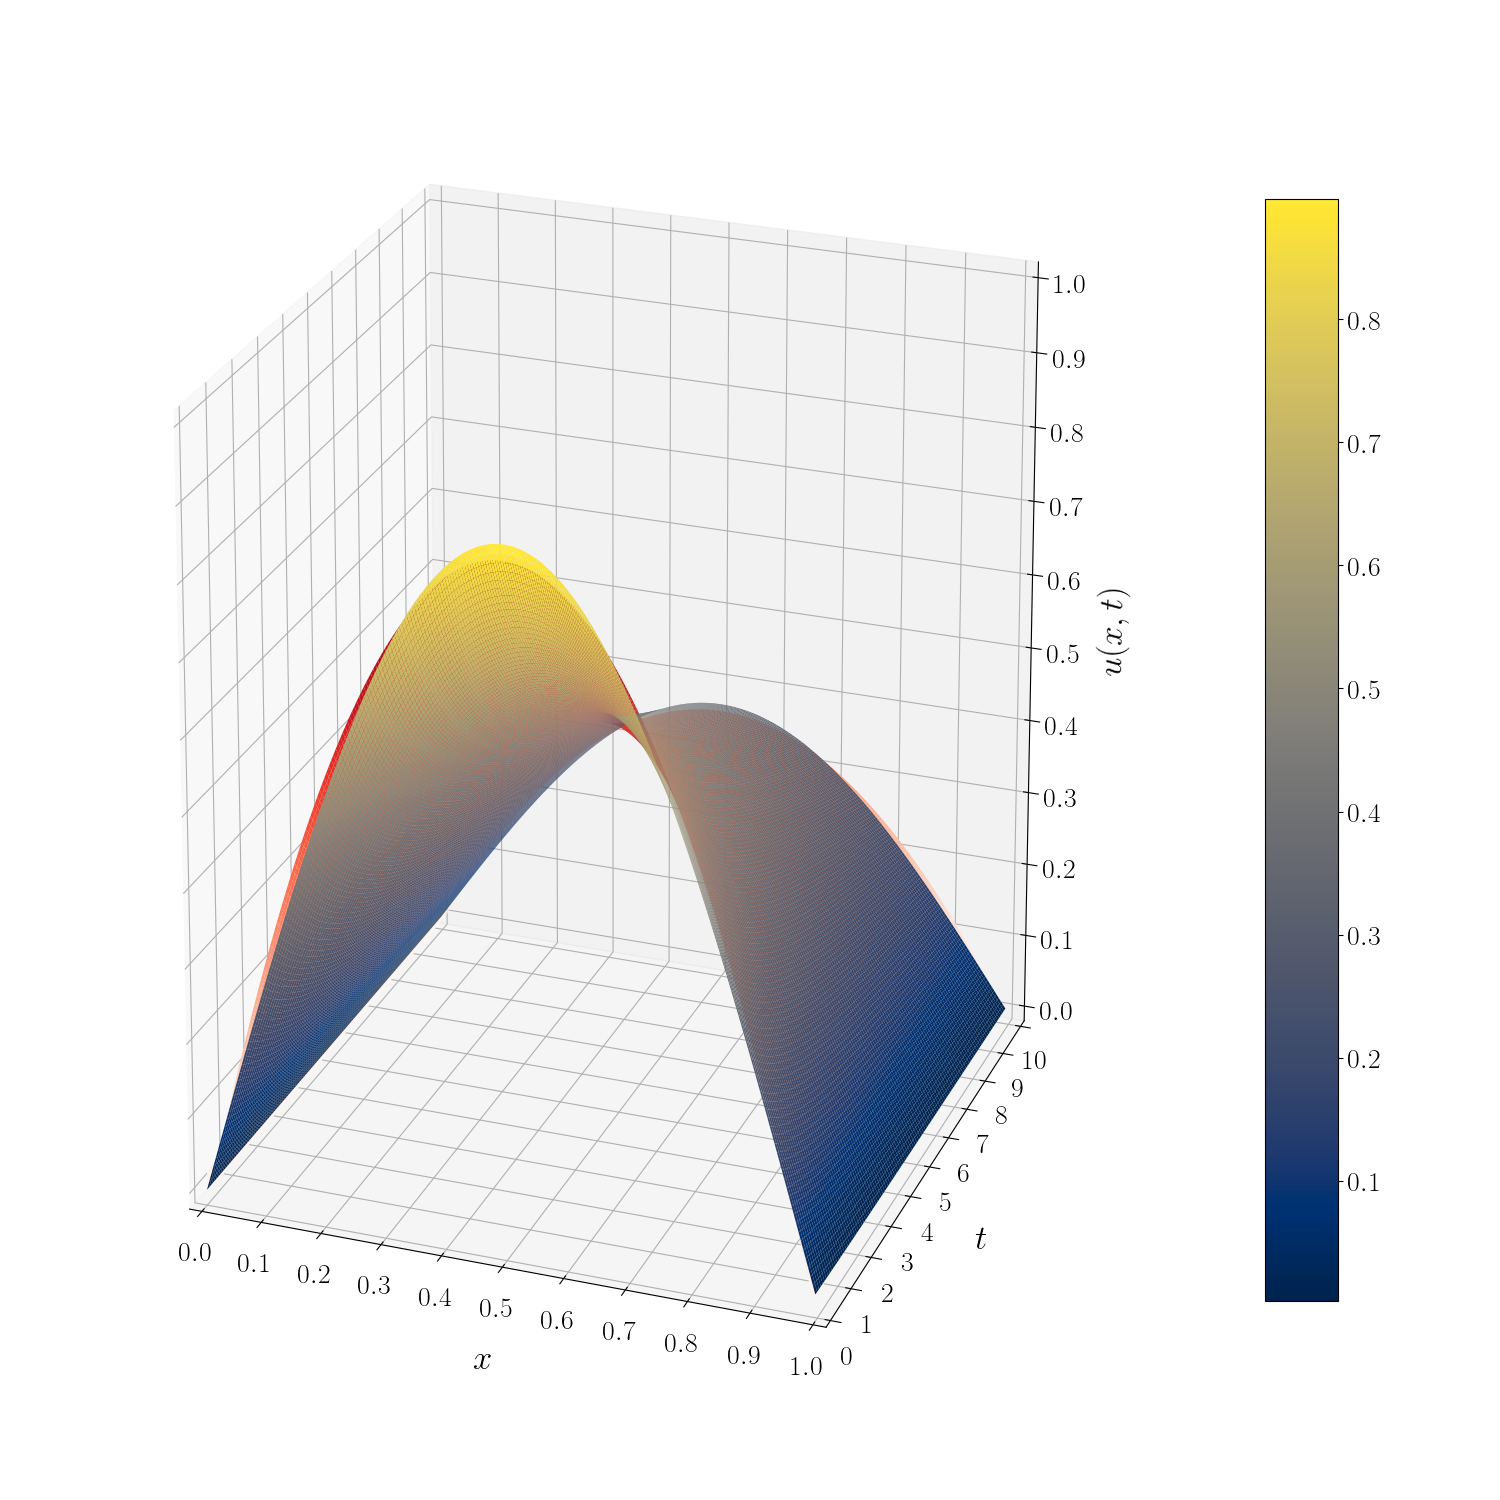
\includegraphics[width=.9\textwidth]{burgers_equation/stochastic/numerical_experiments/figures/Numerical_Solution_Stochastic.png}
		\caption{Numerical solutions for (\ref{burgers_stochastic2}) with initial conditions $x(\xi)$ and $y(\xi)$.}
		\label{Stochastic_Solutions}	
	\end{figure}
\newpage
	\begin{figure}[H]	
	\centering
		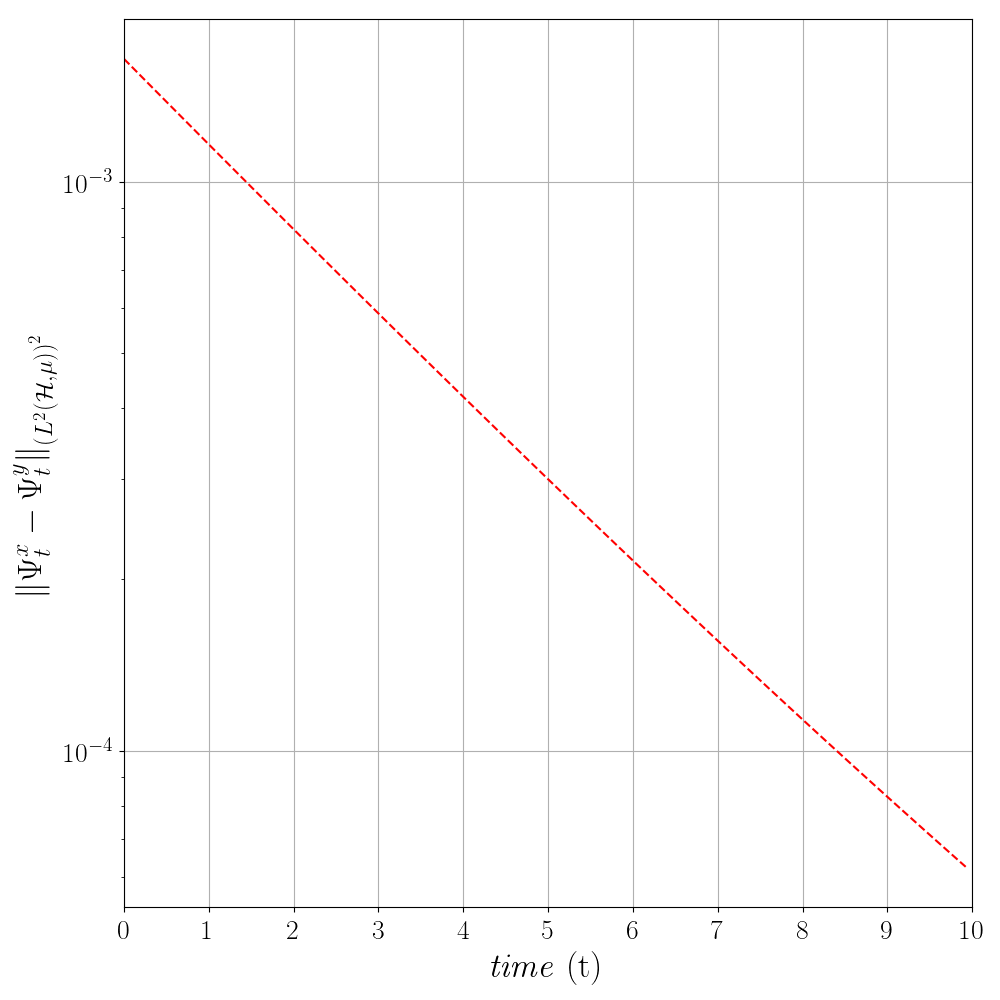
\includegraphics[width=.7\textwidth]{burgers_equation/stochastic/numerical_experiments/figures/norms.png}
		\caption{Distance between the numerical solutions for equation (\ref{burgers_stochastic2}) with initial conditions $x(\xi)$, and $y(\xi)$.}
		\label{Continuity}
	\end{figure}